\documentclass[12pt, twoside]{article}
\input{../preamble}

\fancyhead[LE]{\thepage}
\fancyhead[RO]{Name: \hspace{4cm} \,\\ 12th Grade \hspace{2.9cm} \,}
\fancyhead[LO]{La Scuola d'Italia / Dr.\ Huson / IB Math: Probability \\* March 2026}

\begin{document}
\subsubsection*{4.12 Quiz: Probability}
\begin{enumerate}[itemsep=0.1cm]

%--- Problem 1: Venn diagram ---
\item In a survey of 40 students, 22 own a bicycle and 15 own a scooter.
Seven students own both, as shown in the following Venn diagram.
The values $\boldsymbol{p}$ and $\boldsymbol{q}$ represent numbers of students.

\begin{center}
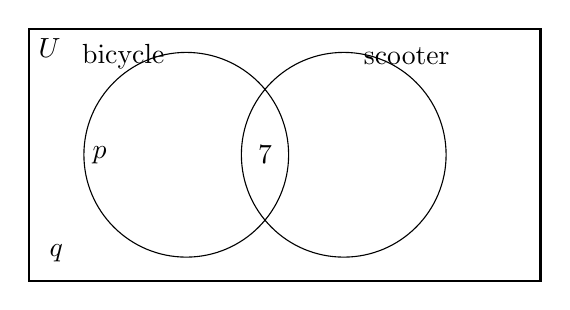
\begin{tikzpicture}
  \draw[thick] (0,0) rectangle (6.5,3.2);
  \node[anchor=north west] at (0,3.2) {$U$};
  \draw (2.0,1.6) circle (1.3cm);
  \node at (1.2,2.85) {bicycle};
  \draw (4.0,1.6) circle (1.3cm);
  \node at (4.8,2.85) {scooter};
  \node at (0.9,1.6) {$p$};
  \node at (3.0,1.6) {$7$};
  \node at (0.35,0.35) {$q$};
\end{tikzpicture}
\end{center}

\begin{enumerate}[itemsep=0.25cm]
  \item Find the value of $\boldsymbol{p}$. \hfill [1]
  \item Find the value of $\boldsymbol{q}$. \hfill [1]
  \item A student is chosen at random. Find the probability that the student
        owns a scooter but not a bicycle. \hfill [2]
\end{enumerate}

\begin{tikzpicture}
  \draw (0,0) rectangle (15.5,5);
  \foreach \y in {1,2,3,4} \draw[dotted] (0.5,\y)--(15,\y);
\end{tikzpicture}

%--- Problem 2: Mutually exclusive ---
\item Events $A$ and $B$ are mutually exclusive with
$\mathrm{P}(A) = 0.55$ and $\mathrm{P}(B) = 0.15$.

\begin{enumerate}[itemsep=0.25cm]
  \item Write down $\mathrm{P}(A \cap B)$. \hfill [1]
  \item Find $\mathrm{P}(A \cup B)$. \hfill [2]
\end{enumerate}

\begin{tikzpicture}
  \draw (0,0) rectangle (15.5,4);
  \foreach \y in {1,2,3} \draw[dotted] (0.5,\y)--(15,\y);
\end{tikzpicture}

\newpage

%--- Problem 3: Fully-labeled Venn diagram ---
\item In a group of 40 students, some play football ($F$) and some play basketball ($B$).
Eight students play neither sport. This information is shown in the following Venn diagram.

\begin{center}
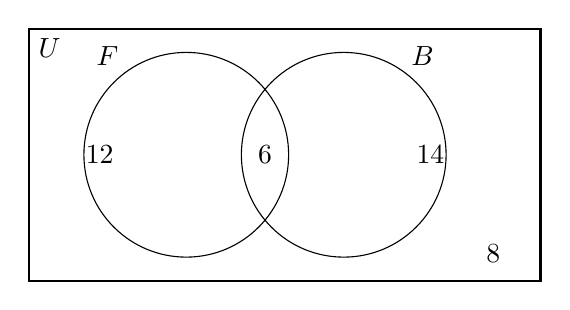
\begin{tikzpicture}
  \draw[thick] (0,0) rectangle (6.5,3.2);
  \node[anchor=north west] at (0,3.2) {$U$};
  \draw (2.0,1.6) circle (1.3cm);
  \node at (1.0,2.85) {$F$};
  \draw (4.0,1.6) circle (1.3cm);
  \node at (5.0,2.85) {$B$};
  \node at (0.9,1.6) {$12$};
  \node at (3.0,1.6) {$6$};
  \node at (5.1,1.6) {$14$};
  \node at (5.9,0.35) {$8$};
\end{tikzpicture}
\end{center}

\begin{enumerate}[itemsep=0.25cm]
  \item Write down the number of students in the group who play football. \hfill [2]
  \item One student from the group is chosen at random. Find the probability that
  \begin{enumerate}[label=(\roman*), itemsep=0.25cm]
    \item the student does not play football;
    \item the student plays football or basketball, but not both. \hfill [4]
  \end{enumerate}
\end{enumerate}

\begin{tikzpicture}
  \draw (0,0) rectangle (15.5,10);
  \foreach \y in {1,2,...,9} \draw[dotted] (0.5,\y)--(15,\y);
\end{tikzpicture}

\end{enumerate}
\end{document}

Solutions
Problem 1 — Venn diagram: 40 students, bicycle/scooter, 7 own both
  - (a) p = 22 - 7 = 15
  - (b) q = 40 - (22 + 15 - 7) = 40 - 30 = 10
  - (c) P(scooter only) = 8/40 = 0.2

Problem 2 — Mutually exclusive: P(A) = 0.55, P(B) = 0.15
  - (a) P(A ∩ B) = 0  (definition of mutually exclusive)
  - (b) P(A ∪ B) = 0.55 + 0.15 = 0.70

Problem 3 — Fully-labeled Venn diagram: 40 students, football/basketball
  - (a) Number who play football = 12 + 6 = 18
  - (b)(i)  P(not football) = (14 + 8)/40 = 22/40 = 0.55
  - (b)(ii) P(football or basketball, not both) = (12 + 14)/40 = 26/40 = 0.65
